\chapter{Discussion}
\label{ch:discussion}
This chapter is dedicated to summarizing and discussing our thesis. Each section is covers a specific research questions and shows how our findings helped shape the answers to the questions posed. The research questions are discussed in the order they were posed in Section~\ref{sec:researchQuestions}. The chapter finishes with looking at how our research questions can be applied to other media.

\section{Scenarios and User Group}
Our first research question states:
\begin{quote}
\textit{What are the relevant scenarios for visual presentation of accelerometer data in physical therapy, from the physiotherapist's perspective?}
\end{quote}

Initially we designed the first prototype for two scenarios:
\begin{table}[h!]
  \begin{tabular}{|c|p{10cm}|}
    \hline
    \textbf{Id} & \textbf{Scenario} \\ \hline
    IS-1 & Mapping the activity level of patients \\ \hline
    IS-2 & In consultation with patients \\ \hline
  \end{tabular}
  \caption[Initial scenarios.]{Table showing the initial scenarios.}
\end{table}

These are the most obvious scenarios for the system. After the first and second focus group three more scenarios emerged, as well as the initial ones being heavily modified. The new and reviewed scenarios can be found in Table~\ref{tab:scenariosFinal1}.

\begin{table}[h!]
  \begin{tabular}{|c|p{10cm}|}
    \hline
    \textbf{Id} & \textbf{Scenario} \\ \hline
    S2-1 & When analysing patients activity level, either individually or in cooperation with occupational therapists or other physiotherapists. \\ \hline
    S2-2 & In consultation with the patient. \\ \hline
    S2-3 & In communication with nursing homes and home care personnel. \\ \hline
    S2-4 & In consultation with next of kin. \\ \hline
    S2-5 & For educational purposes. \\ \hline
  \end{tabular}
  \caption[Scenarios after the second focus group.]{Table showing the scenarios after the second focus group.}
  \label{tab:scenariosFinal1}
\end{table}

The first scenario was changed to include the cooperation with other physiotherapists or occupational therapists. During the second focus group the participants informed us that if they were to discuss a patient with colleagues it would usually be with an occupational therapist or in rare cases another physiotherapist. Normally the physiotherapists would not consult their colleagues about specific patients. 

% REVEIW
Currently a set of exercises and the physiotherapists subjective opinion of the patient are the only ways physiotherapists can map the patient's activity level. With sensor technology such as the activPAL and detailed visualizations to display the sensor data, physiotherapists can get a much more accurate picture of patients activity patterns. This would be a great help when creating a treatment plan for the patients, as they can pinpoint when the patient is least active, the length of intervals of sedentary behaviour, if the patient is active during the night, etc. This valuable information is hard or impossible to acquire with the current methods for mapping patient activity.

The second scenario is one of the most important uses the system can have. Showing the visualizations to the patient can be useful in many cases, for example when explaining to the patient their current activity level, and why exercise or more movement is needed. Visualizations are also useful for motivating the patients, by showing them detailed figures on their progress they can see that the exercises they have to do are helping. Many of the patients treated by the physiotherapists who working for Trondheim Kommune are elderly and not as cognitively capable as they once were, especially those living in nursing homes. The participants estimated that about half of their patients would be capable of understanding the visualizations presented. Some of the visualizations are very simple and could probably be used on a larger patient group, but less detailed visualizations will often be less helpful. 

For patients that can not understand the visualizations themselves, scenario 3 and 4 become increasingly important. Patients living in nursing homes receive help throughout the day, and are unable to preform trivial tasks like making breakfast or go shopping. During the focus groups the participants were concerned that when patients stopped doing such tasks the little activity they previously had was lost, leading to an inactive and unhealthy lifestyle. To combat this, the participants were eager to be able to monitor the activity of such patients, and in cooperation with personnel working there increase the activity of the patients. 

In many cases the patients next of kin can be consulted after or during evaluation of the patients activity level. Next of kin can be an important motivator for the patient, and help the physiotherapists persuade patients to follow the agreed upon treatment plan. Next of kin are normally interested in the well being of the patient. The system can be used to help them get a picture of the overall activity level of the patient as well as how they are progressing if they have started treatment. In cases where the patients are not capable of understanding the visualizations themselves, it can be helpful to show them to the next of kin to give them an idea of what needs for the patient to achieve an acceptable level of activity. Next of kin are able to spend more time with the patient than the physiotherapists and can thus help the patient achieve their goals by motivating them to take a walk or perform household tasks.

The focus group participants believed that the visualizations could be helpful for educational purposes. A project currently ongoing in Trondheim is teaching home care personnel how to preform physiotherapy exercises with their patients. This will give elderly patients living at home better access to help when they have been asked to preform exercises by the physiotherapists. The participants of the focus groups suggested that visualizations could be used in training of both physiotherapy students and home care personnel to show them how preforming different exercises can help improve the overall activity of the patient.

\section{Requirements}
The second research question states:
\begin{quote}
\textit{What are the functional and user experience requirements for visualizations of accelerometer data in the scenarios identified by the physiotherapists?}
\end{quote}

Requirements gathering is an important part of any software development project. Because the initial requirements were created in cooperation with a domain expert and not the participants of the focus groups we saw a lot of changes to the requirements after the first focus group. The requirements aim to give instructions as to what types of visualizations should be created, and with all the feedback and changes to the visualizations after the first focus group, it is not surprising that the requirements also changed substantially.

\begin{table}[h!]
  \begin{center}
  \begin{tabular}{|c|p{12cm}|}
    \hline
      \textbf{Id} & \textbf{Requirement} \\ \hline
    \multicolumn{2}{|l|}{The visualizations should \ldots} \\ \hline
      IR-1 & give an overview of the week \\ \hline
      IR-2 & give a summary of the daily activity \\ \hline
      IR-3 & show the activity level for each hour of every day \\ \hline
      IR-4 & let the user compare hours from multiple days \\ \hline
      IR-5 & show the activity level for each minute of every day \\ \hline
      IR-6 & let the user compare minutes from multiple days \\ \hline
      IR-7 & let the user identify patients that are active during the night \\ \hline
  \end{tabular}
  \end{center}
  \caption[Initial requirements]{Initial requirements.}
  \label{tab:initReq}
\end{table}

Looking at the initial requirements in Table~\ref{tab:initReq}, requirements IR-5 and IR-6 were removed after talking to the physiotherapists in focus group 1. Visualizations showing the continuous activity pattern of users was seen as too detailed to be useful. The participants also felt that it was too hard to see the activity, because it was hidden by the inactive and standing periods. The other initial requirements were modified and rephrased, but still remain in the R1-version of the requirements, see Table~\ref{tab:f1Req}. 

Requirement R1-5 is a direct results of comments from the participants during the first focus group. They stated that one of the most useful features of the system is the ability to see when during the day the patient is inactive. This can be used to plan activity and exercises to specific hours of the day when the physiotherapists knows the patient will most likely be inactive. Having this type of detailed information can help the physiotherapists create an even more specific treatment plan for the patient, and possibly increasing the quality and effectiveness of the treatment. A functionality that was requested during the first focus group was the ability to set goals. The physiotherapists had a hard time identifying whether the patients data represented an active or an inactive person without comparing the data to some fixed goal. To satisfy this request, R1-6 was a new requirement added after focus group 1. IR-1 was also changed to R1-1 to make the classification in the overview charts take into consideration patient goals.

Another interesting addition was R1-9, which states that the visualizations should have printable greyscale versions. It was surprising to hear about how few technological aids were available to the physiotherapists working for Trondheim Kommune (municipality of Trondheim). For scenarios where the physiotherapists only have access to grayscale printouts, important system functionality such as interactivity, will be lost.

\begin{table}[h!]
  \begin{center}
  \begin{tabular}{|c|p{12cm}|}
    \hline
      \textbf{Id} & \textbf{Requirement} \\ \hline
    \multicolumn{2}{|l|}{The visualizations should \ldots} \\ \hline
      R1-1 & give the user an overview of the week where the days are classified by national or personal goals \\ \hline
      R1-2 & show the activity level for each hour of the day \\ \hline
      R1-3 & make it simple to identify periods of inactivity \\ \hline
      R1-4 & make it possible to compare multiple days \\ \hline
      R1-5 & make it easy to identify hours of the day where activity can be added \\ \hline
      R1-6 & show the activity level compared to national or personal goals \\ \hline
      R1-7 & let the user identify patients that are active during the night \\ \hline
      R1-8 & let the user compare two separate weeks to see the patients progress \\ \hline
      R1-9 & be printable in grayscale \\ \hline
  \end{tabular}
  \end{center}
  \caption[Functional requirements after the first focus group.]{Functional requirements from the first focus group.}
  \label{tab:f1Req}
\end{table}

Two requirements were added after the second focus group, F2-15 and R2-16, see Table~\ref{tab:f2Req}. R2-15 is a clarification of the first requirement. The participants felt that there was no requirement specifying the need for aggregated charts, and R2-15 was therefore added. Another functionality that was requested was the ability to toggle nighttime on and off. In the first focus group many of the participants felt that including nighttime, especially in the aggregated charts, made the inactive part of the chart too large. Nighttime was therefore removed for some of these graphs in the second prototype. However, the participants were now uncertain as to what period of the night had been removed. It was therefore suggested that that the user should be able to toggle nighttime on and off, so that in cases where it would be helpful to see the entire dataset this option would still be available. The participants also wanted the ability to define the time interval that should be considered  nighttime. For patients living in institutions nighttime is similar for all the patients, but for patients living at home nighttime might differ from patient to patient.

\begin{table}[h!]
  \begin{center}
  \begin{tabular}{|c|p{12cm}|}
    \hline
      \textbf{Id} & \textbf{Requirement} \\ \hline
    \multicolumn{2}{|l|}{The visualizations should \ldots} \\ \hline
      R2-1 & give the user an overview of the week where the days are classified by national recommendations or personal goals \\ \hline
      R2-2 & show the activity level for each hour of the day \\ \hline
      R2-3 & make it easy to identify the length of activity intervals \\ \hline
      R2-4 & make it possible to compare multiple days \\ \hline
      R2-5 & make it easy to identify hours of the day where activity can be added \\ \hline
      R2-6 & show the activity level compared to national or personal goals \\ \hline
      R2-7 & let the user identify patients that are active during the night \\ \hline
      R2-8 & let the user compare two separate weeks to see the patients progress \\ \hline
      R2-9 & should be printable in grayscale \\ \hline
      R2-15 & show the activity distribution for a day (sedentary, standing, walking) \\ \hline
      R2-16 & allow the users to toggle if nighttime should be included or not \\ \hline
  \end{tabular}
  \end{center}
  \caption[Functional requirements after the second focus group.]{Functional requirements from the second focus group.}
  \label{tab:f2Req}
\end{table}

\begin{table}[h!]
  \begin{center}
  \begin{tabular}{|c|p{12cm}|}
    \hline
      \textbf{Id} & \textbf{Requirement} \\ \hline
    \multicolumn{2}{|l|}{The visualizations should \ldots} \\ \hline
      F2-10 & not be judgemental towards the patients activity level \\ \hline
      F2-11 & should be honest about the patients activity level \\ \hline
      F2-12 & should motivate the patient to be more active \\ \hline
      F2-13 & should be intuitive and easy to understand for the user and third parties \\ \hline
      F2-14 & be easy to explain to cognitively capable patients \\ \hline
  \end{tabular}
  \end{center}
  \caption[User experience requirements after the second focus group.]{User experience requirements from the second focus group.}
  \label{tab:f2ReqUx}
\end{table}

Talking with the physiotherapists also gave us the ability to explore \gls{ux} requirements for the system, see Table~\ref{tab:f2ReqUx}. The \gls{ux} requirements we created are important to keep in mind when creating visualizations, these requirements may not be intuitive without understanding how the physiotherapists work. One of the first responses we got when going through the visualizations in the first focus group, was that the visualization had a negative attitude. For example using smilies to represent the classifications could demotivate and be judgemental towards the patient. These are issues we did not consider when first creating prototype 1. The physiotherapists also stressed that though the visualizations should not be judgemental it was just as important that they did not lie. They should give the patient an honest representation of their activity level, but without making the patient feel hopeless. Many patients are prone to give up before they have even started, and it is paramount that the visualizations do not contribute in discouraging the patient.

Motivating patients is another important \gls{ux} requirements. One of the physiotherapists pointed out that patients like to see quantitative data to show that they are improving. Progress can be slow and hard to notice from day to day. This can in many cases discourage patients from doing their exercises. Seeing quantitative proof that one is constantly improving, can be a powerful motivational tool, as it gives the patient a reward for following the exercise plan. One of the physiotherapists also stated that patients tend to trust more in statistics and diagrams than they do in the qualitative judgement from the physiotherapists alone. Using visualizations in their work can therefore help them persuade patients who are otherwise distrustful or feel that the treatment plan is ineffective or pointless. For the patients to be motivated by the visualizations, they need to be able to understand them, and this is covered by the R2-12 requirement. 

\section{Visualizations}
The final research question is concerned with visualizations and states:
\begin{quote}
  \textit{What are the preferred visualizations by the physiotherapists for the scenarios and requirements?}
\end{quote}

During the creation of the first paper sketches we created three groups of visualizations: overview charts, aggregated charts and timeline charts. The overview charts were designed to let the user to quickly get an overview of the week as a whole. For the first prototype two such overviews were created, U1 and U2. U2 was quickly discarded because it contained too many details which only confused the participants of the first focus group. U1 was kept in the second prototype and received positive feedback by the participants in the second focus group. U1 uses personal or national goals to classify each day into one of three categories. Making U1 very easy to understand, and one of the physiotherapists stated that because it was so easy to understand this might be one of the visualizations that would be shown to the patients. The visualization also works well for printouts, both colour and grayscale. To further improve U1 an indication as to what the current goal is set to should be added, such information would help the physiotherapist and patient understand what the different classifications correspond to.

\begin{figure}[h!]
  \centering
  \begin{subfigure}[b]{0.49\textwidth}
    \centering
    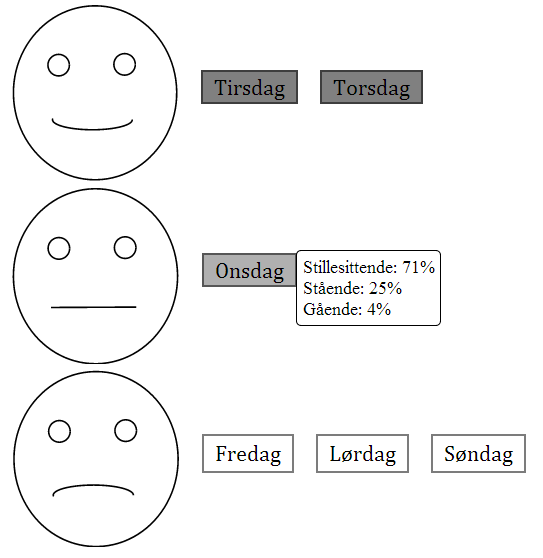
\includegraphics[width=0.5\textwidth]{u1First.png}
    \caption{U1 in prototype 1.}
  \end{subfigure}
  \begin{subfigure}[b]{0.29\textwidth}
    \centering
    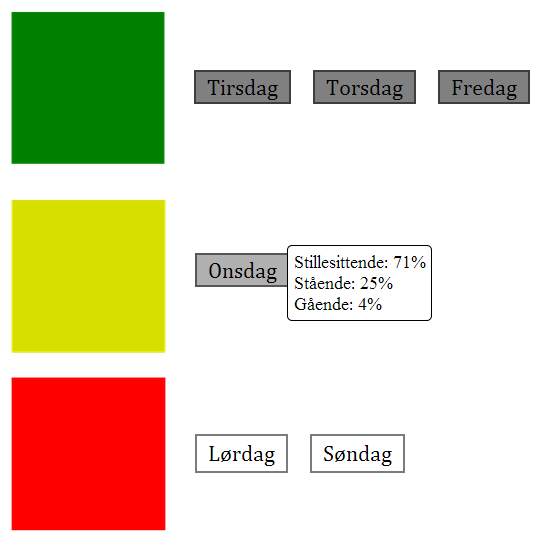
\includegraphics[width=\textwidth]{u1Second.png}
    \caption{U1 in prototype 2.}
  \end{subfigure} 
  \caption{First and second version of U1}
  \label{fig:uComparison}
\end{figure}

The aggregated charts sum up the day to show the distribution of different types of activity. Initially there were three types of aggregated charts: F1, F2 and F3. F1 and F2 were combined for the second prototype to become a standard pie chart with three slices, one for each activity type. The pie chart also contains illustrations that show what type of activity each slice corresponds to. Pie charts are easy to understand because most people will have seen them before, know what they mean and know how to read them. F1 can therefore also be shown to the patient when explaining their current level of activity. F3 is a bubble chart, most people will not have seen this type of chart before and it is not as intuitive as F1. The physiotherapists like the chart because it can be used to see intervals of activity, for example the longest walk a patient took during a day. This type of graph would most likely not be shown to the patients as most of them would not understand it. F3 could be used in communication with nursing homes and home care personnel, for example if the patient needs to be walking for longer periods of time not just in small intervals. 

\begin{figure}[h!]
  \centering
  \begin{subfigure}[b]{1\textwidth}
    \centering
    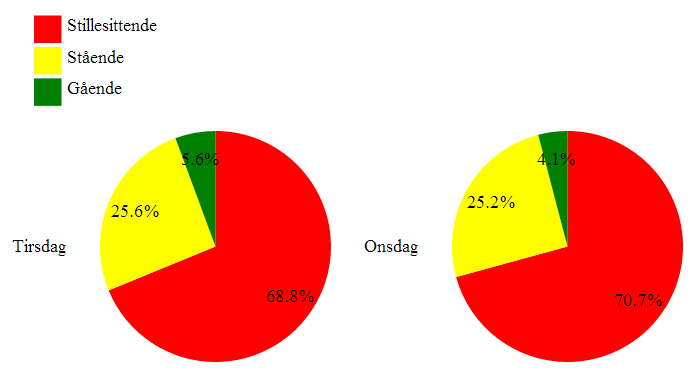
\includegraphics[width=0.5\textwidth]{f1First.png}
    \caption{F1 in prototype 1.}
  \end{subfigure}
  \\
  \begin{subfigure}[b]{0.6\textwidth}
    \centering
    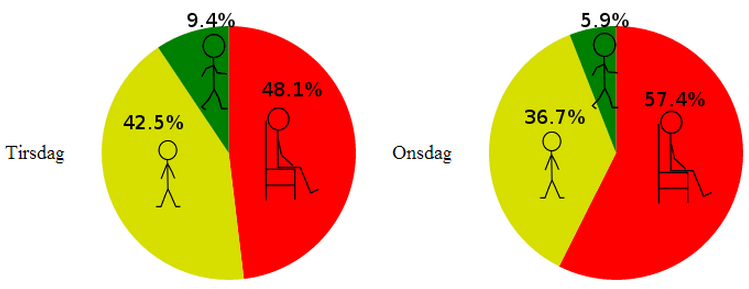
\includegraphics[width=\textwidth]{f1Second.png}
    \caption{F1 in prototype 2.}
  \end{subfigure} 
  \caption{First and second version of F1}
  \label{fig:fComparison}
\end{figure} 

Timeline charts show the activity during the day continuously or in aggregated blocks. Four timeline charts were initially created: T1, T2, T3 and T4. T2, T3 and T4 showed activity during the day minute for minute without aggregating it into hours. These visualizations were discarded because the physiotherapists felt that the amount of detail was unnecessary and only made the visualizations harder to read and less useful. T1 uses 24 blocks where the activity of each hour were aggregated and displayed using a gradient. T1 was the preferred graph, as it was easy to get an overview of the day as a whole, as well as the entire week by stacking multiple days on top of each other. This meant that the physiotherapists could easily get an overview of the overall activity pattern of the patient. This made it easy to find inactive hours where the patient could be motivated to do exercises or move around. Noticing patients who are active during the night is also easy due to the way hours with activity gain increase in colour intensity. During the focus group one of the physiotherapists told us that a common problem for elderly patients is that they can not sleep and therefore walk around during the night, leading to less activity during the day. Such patterns can easily be detected using T1, as an example we were able to see from the example data that the patient would walk for a few minutes most nights at 4 am, probably to go to the toilet.

\begin{figure}[h!]
  \centering
  \begin{subfigure}[b]{1\textwidth}
    \centering
    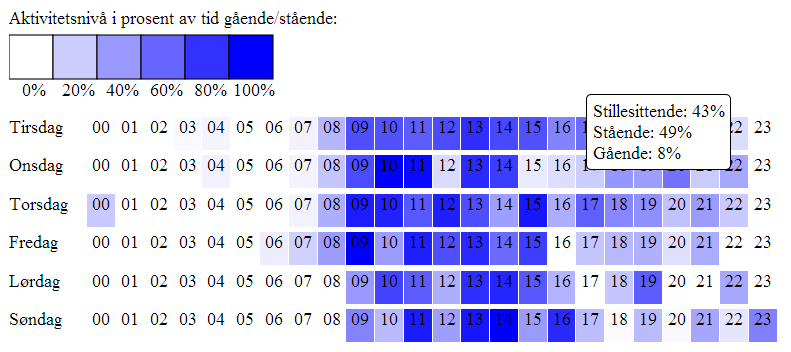
\includegraphics[width=0.5\textwidth]{t1FirstWeek.png}
    \caption{T1 week view in prototype 1.}
  \end{subfigure}
  \\
  \begin{subfigure}[b]{0.6\textwidth}
    \centering
    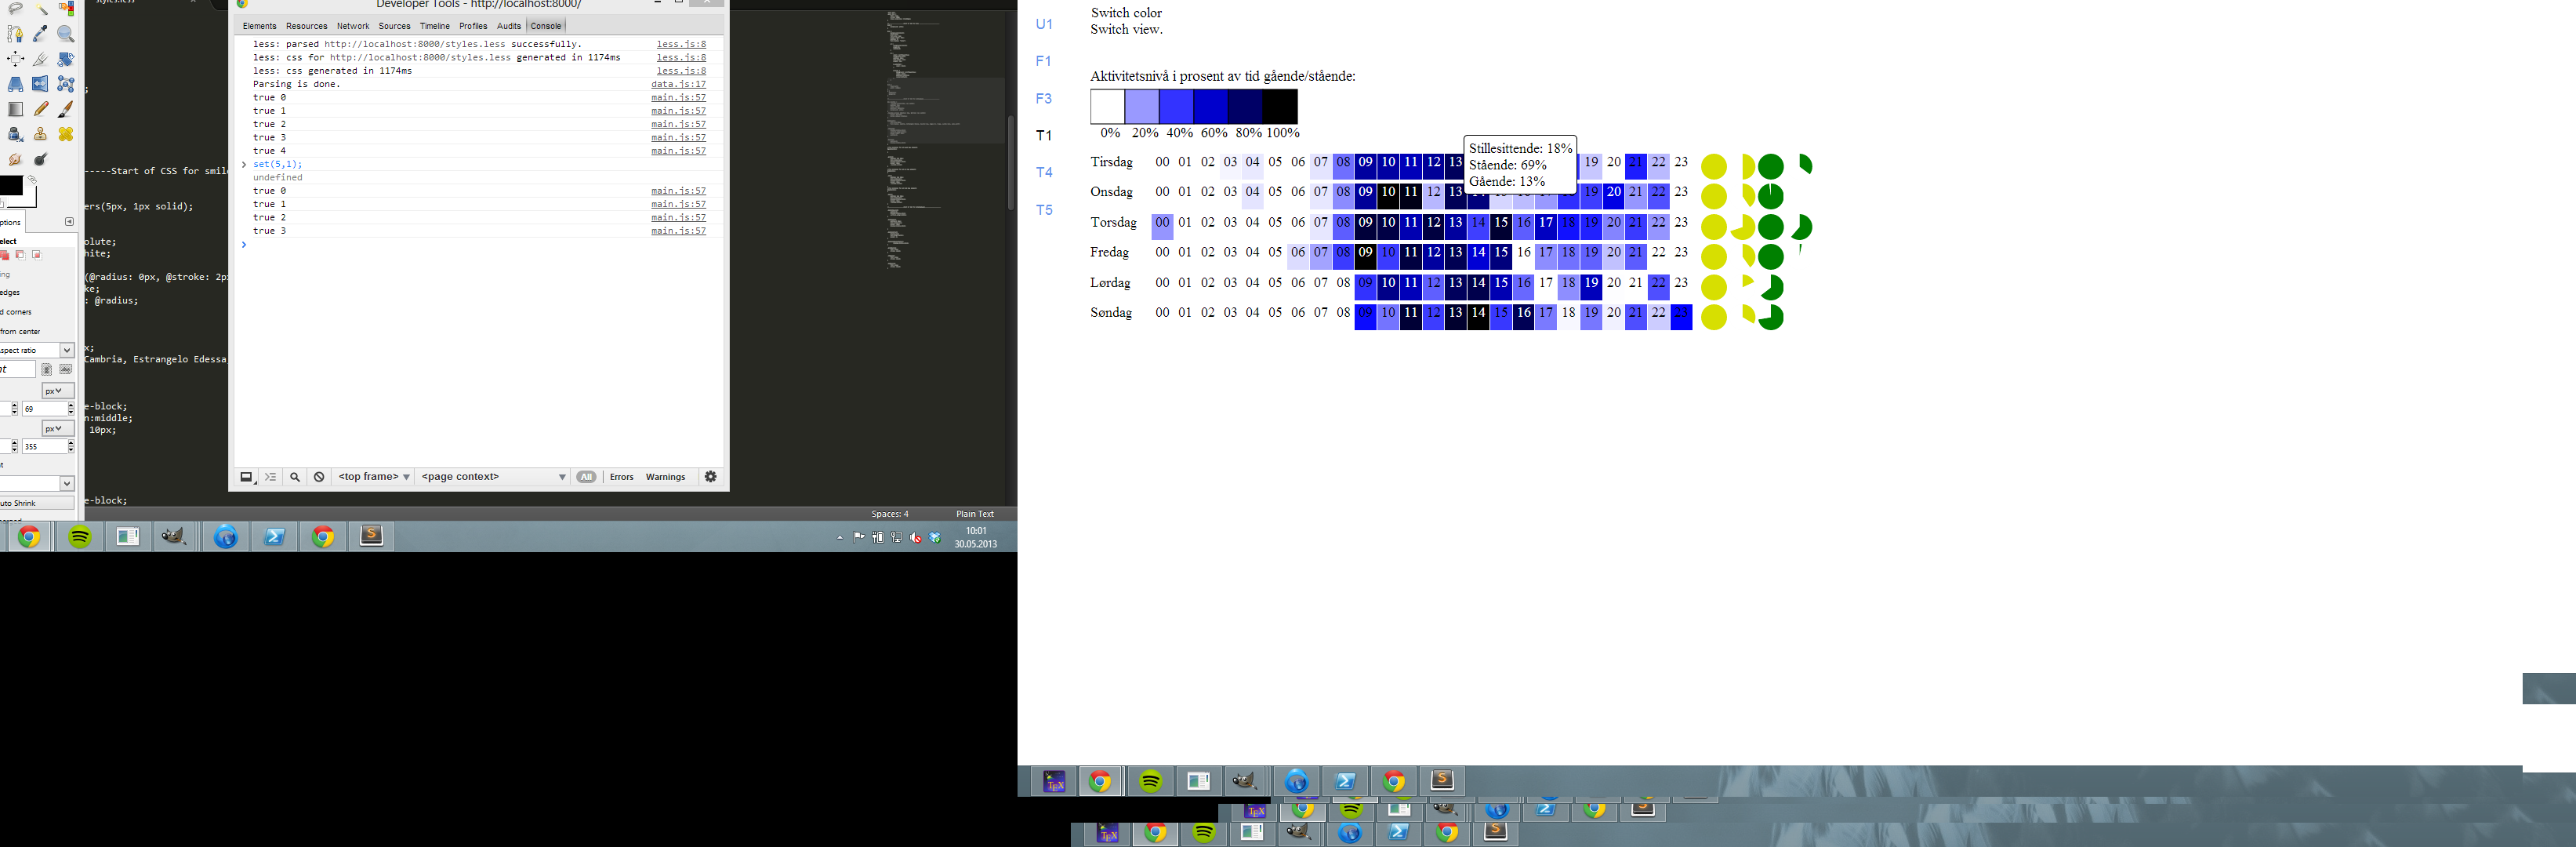
\includegraphics[width=\textwidth]{t1SecondWeek.png}
    \caption{T1 week view in prototype 2.}
  \end{subfigure} 
  \caption{First and second version of T1}
  \label{fig:tComparison}
\end{figure} 

Though the T1 is not very hard to understand,  but it requires high cognitive capability than U1 and F1, therefore it could most likely only be displayed to the more cognitively capable patients. Another issue with T1 is that the gradient colours it uses do not translate well when printed. T5 was created for the second prototype and like T1 divides the day into 24 blocks, but instead of using gradient to display the distribution of activity stacked bars are used. This visualization is also similar to the chart used in the activPAL software, but in T5 seated or lying activity is not displayed with bars, this increases the readability of the graph. Despite this T1 was still the favourite because it is easier to stack days on top of each other when using gradient colouring instead of stack bars to represent activity within an hour. One benefit of T5 compared to T1 is that is works much better when printed, as it does not rely on a colour scale.

For the second prototype personal and national goals were added. This addition was heavily requested by the physiotherapists after the first focus group. To show how the patient's activity compared to the goals that had been set, a visualization called goal circles was created. As the name suggests the visualization uses circles to display how far the patient is from reaching the goal or how far they have exceeded it. The goal circles were appended to each day of T1 and T5. The participants of the second focus group did not like this, and felt that the goal circles should have been its own visualization, used only to see if the patient were reaching the goals set. The goal circles are also intuitive and easy to understand, and they could be shown to some patients. An issue with the goal circles is that they do not display the currently set goals, all graphs using the goals should display what the current goals are set to. Goals are an important motivational factor when patients are attempting to become more active.

Table~\ref{tab:reqSat} shows which requirements are satisfied by each visualization. Each row represents a visualization and each column corresponds to a functional requirement. A -- means that the requirement is not satisfied by the visualization and a + means that it is satisfied. As we can see there are two requirements, R2-8 and R2-16, that are not covered by any of the visualizations. R2-8 says that the user should be able to compare two different weeks to see if there has been progress. Comparing weeks is important for the system to function as a motivational tool. This requirement was suggested after focus group 1, but was not implemented due to lack of time. R2-16 states that the visualizations should let the user toggle nighttime on and off. This requirement was suggested in focus group 2 and was therefore not implemented for prototype 2.

\begin{table}[h!]
  \centering
  \begin{tabular}{|c|c|c|c|c|c|c|c|c|c|c|c|}
    \hline
    & R2-1 & R2-2 & R2-3 & R2-4 & R2-5 & R2-6 & R2-7 & R2-8 & R2-9 & R2-15 & R2-16 \\ \hline
    U1 & + & -- & -- & + & -- & -- & -- & -- & + & -- & -- \\ \hline
    F1 & -- & -- & -- & + & -- & -- & -- & -- & + & + & -- \\ \hline
    F3 & -- & -- & + & -- & + & -- & -- & -- & -- & + & -- \\ \hline
    T1 & -- & + & -- & + & + & + & + & -- & -- & -- & -- \\ \hline
    T5 & -- & + & -- & + & + & + & + & -- & + & -- & -- \\ \hline
  \end{tabular}
  \caption[Requirements and visualizations]{The table shows which requirements each visualization satisfies.}
  \label{tab:reqSat}
\end{table} 

Table~\ref{tab:scenSet}, see below, shows which visualizations satisfy each scenario. The first scenario is physiotherapists using the visualizations to analyse the patients activity level. In such cases all the visualizations can be utilized to get the best overview of the patients activity situation. For the most part T1 and T5 would be used as these give the best overview of the week and it is easy to identify where more activity can be added. 

\begin{table}[h!]
  \centering
  \begin{tabular}{|c|c|c|c|c|c|}
    \hline
       & S2-1 & S2-2 & S2-3 & S2-4 & S2-5 \\ \hline
    U1 & +  & +  & -- & +  & +  \\ \hline
    F1 & +  & +  & +  & +  & +  \\ \hline
    F3 & +  & -- & +  & -- & +  \\ \hline
    T1 & +  & -- & +  & -- & +  \\ \hline
    T5 & +  & +  & +  & +  & +  \\ \hline
  \end{tabular}
  \caption[Scenarios and visualizations]{Table showing which scenarios each visualization satisfies.}
  \label{tab:scenSet}
\end{table}

The second scenario is using the visualizations in consultation with the patient. For many of the patients it will not be possible to show any of the visualizations, but for those that are cognitively capable most of the visualizations can be used. F3 was excluded because it can be hard to explain, and it does not contain information that is critical to convey to the patient. T1 will not work on paper printouts, but could be used if the physiotherapists have access to laptops or tablets.

The third scenario is concerned with communication with nursing homes and home care personnel. All visualizations can be used for this purpose, but U1 will probably not be effective in conveying information of interest and was therefore excluded. F3 and T1 can be helpful tools when discussing the activity level of patients with other health care personnel.

Consulting the next of kin is the fourth scenario. Most visualizations can be used for this purpose. F3 was excluded because it will probably be more confusing than helpful in explaining the patients current activity level. T1 was also excluded as it will does not work well for printouts.

For educational purposes, S2-5, all the visualizations can be used. Each visualization serves different functions and to get a complete overview of the patients activity level it can be useful to look at multiple visualizations. T1 and F1 are probably the best for this purpose. F3 can be used in situations where it is helpful to see the length of different type of activity.

\section{Visual Variables}
Five visualizations were accepted by the physiotherapists: U1, F1, F3, T1 and T5. The different visualizations make use of different visual variables, see Section~\ref{sec:visualVariables}. U1, as seen in Figure~\ref{fig:uSecond}, uses position, size, colour and value (a type of visual variable) to illustrate how the patient fared compared to the set goals. The vertical position of each day, in combination with the coloured square, is used to show how each day is classified. Position is associative, which means that the position of the elements makes humans look at each horizontal level as a group of elements. Elements on the same level also have the same colour gradient, which increases this association. Because every rectangle representing a day has the same size, it is easy to compare how many days there are in each horizontal level by looking at how long it is. 

The aggregated charts F1 and F3, see Figure~\ref{fig:aggCharts}, make use of the visual variables size and colour. F1 uses the quantitative characteristic of size to show the distribution of different types of activity for a day. F3 can also be used to show the distribution of each type of activity, by summing the size of all the balls for each colour, but the main function of F3 is to show the interval length of each activity event using the size of each ball. The different types of activity is distinguished by the selective property of colours. F3 also uses the associative characteristics of colour and position to group balls corresponding to the same activity together. One possible drawback with using the area of balls to represent the length of an interval, is that human often tend to think that the area of the circle is proportional to the radius, this is not the case. Because this relationship is not proportional, it is much harder to compare the area of two circles than, for example, the length of two lines.

The most popular visualization was T1, see Figure~\ref{fig:t1}. It uses the position of elements to represent the hour of the day that each block corresponds to, and the value to represent the amount of activity for that hour. The advantage of using value is that each day gets very compact, allowing all the days to be stacked on top of each other. This creates a matrix which shows the patients entire week in a lucid way. Using the matrix activity patterns are easy to see. The disadvantage of using value to represent the amount of activity is that it is not qualitative. This means that it is difficult to compare how much more activity there is in one hour compared to another. This is partially solved by the addition of interactivity, since you can hold the cursor over an hour of interest to get the numerical value of activity. T5, see Figure~\ref{fig:t5}, is similar to T1, but uses size to represent the activity for each hour instead of value. This makes it easier to say something about the quantitative values behind each hour, but it also makes it harder to stack the charts on top of each other. For the physiotherapists it seems getting an overview of the week is more important than displaying the exact activity values for each hour. 



\section{Mediums for Presentation of Visualizations}
During the focus groups many different types of devices for displaying the visualizations were discussed. Currently the physiotherapists only have access to grayscale printers. Though adjustments were made to the prototype in order to resolve this problem some of the visualizations, like T1, does not work well on most printers. The loss of interactivity with the charts can also make the visualizations less useful.

One option is to invest in tablets. Tablets are less expensive than laptops and desktop computers and can easily be brought to the patient. A physiotherapist using a tablet will have access to all the visualizations. The touch screen may also give the user the ability to interact with the visualizations. However, our implementation makes use of hover interactivity. This means that information is displayed when the mouse hovers over a certain object. Since a tablet does not use a mouse, the interactivity would need to be changed, for example to clicking/touching objects. Precision can also be problem with tablets. It is hard to select objects that are smaller than ones finger, for example selecting small bubbles in F3 would be nearly impossible using a tablet. F3 would therefore most likely not be very useful if a tablet solution is used. 

Laptops or desktop computers is the solution that was used during the focus group. Laptops can also be brought to the user, and this will give more precision and the ability to use hover selection. Most laptops are usually more powerful than tablets, though performance has not been an issue during the implementation, more complex visualizations might need more processing power than what is currently supported by tablets. Laptops are also faster to write on, and it will be much easier to take notes than on a tablet. The drawback with laptops are that they are more cumbersome to carry, show to patients and often have shorter battery life than tablets. 

It is our opinion that a combined solution, using tablet in the field and laptops or desktop computers in the office, would be optimal. This would give the physiotherapists access to high quality visualization in the field, using them to explain a patient's current activity or to motivate the patient by showing them a visual representation of their progress. The data could also be viewed in more detail and using other, more complex visualization, such as F3, in the office. This solution would give access to all the suggested visualizations and give great flexibility to use the system in all the scenarios.

\section{Certification}
As mentioned in Section~\ref{sec:medicalEquipment} the Norwegian government requires all medical equipment to be certified to ensure that it does not present a danger to the patient or users of the equipment. Software is included in this definition of medical equipment. This means that if the system was to be used in practice, it would first have to be CE-certified. Reading the requirements to get the certificate it is our opinion that the system would pass all the requirements with ease, however we have not studied the certification process in detail.
